\documentclass[xcolor={dvipsnames},aspectratio=169,10pt]{beamer}

% utility packages
\usepackage{multicol}
\usepackage{relsize}
\usepackage{amsthm}
\usepackage[spanish]{babel}
\usepackage{biblatex}
\usepackage{fontawesome}
\usepackage{pgfplots}
\usepackage{enumitem}
\usepackage{empheq}
\usepackage{xcolor}
\usepackage{epigraph}

% better text justifying
\usepackage{microtype}
% justify text inside list environment
% Ref: http://liam0205.me/2017/04/11/justifying-in-beamer-s-lists/
\usepackage{ragged2e}
\makeatletter
\patchcmd{\itemize}{\raggedright}{\justifying}{}{}
\patchcmd{\beamer@enum@}{\raggedright}{\justifying}{}{}
\patchcmd{\@@description}{\raggedright}{\justifying}{}{}
\makeatother

% math related packages
\usepackage{amsmath}
\usepackage[ruled,vlined]{algorithm2e}
\SetAlCapNameFnt{\scriptsize}
\SetAlCapFnt{\scriptsize}
\SetAlFnt{\scriptsize}

% figure related packages
\usepackage{graphicx}
\usepackage[scale=2]{ccicons}
\usepackage{tikz}
\usepackage{tikzpagenodes}
\usetikzlibrary{decorations.pathreplacing}
\usetikzlibrary{positioning}

% table related packages
\usepackage{array}
\usepackage{booktabs}
\usepackage{multirow}
\usepackage{colortbl}
\newcommand{\tabincell}[2]{\begin{tabular}{@{}#1@{}}#2\end{tabular}}

% hyperref setting
\hypersetup{
  unicode,
  psdextra,
  bookmarksnumbered=true,
  bookmarksopen=true,
  bookmarksopenlevel=3,
  bookmarksdepth=4,
  pdfcenterwindow=true,
  pdfstartview={Fit},
  pdfpagemode={FullScreen},
  pdfpagelayout={SinglePage},
}
\usepackage{bookmark}

% beamer theme
\usetheme{metropolis}
\metroset{block=fill,numbering=fraction}

% caption style
\usepackage{subcaption}
\setlength\abovecaptionskip{3pt}
\setbeamerfont{caption}{size=\scriptsize}
\renewcommand{\figurename}{Fig.}
\captionsetup{labelformat=empty,labelsep=none,textfont={bf,it}}

% Ref: https://github.com/gpoore/minted/blob/master/source/minted.dtx
\newenvironment{latexexample}
{\VerbatimEnvironment\begin{VerbatimOut}[gobble=3]{example.out}}{\end{VerbatimOut}%
  \begin{center}
    \begin{minipage}{0.47\linewidth}%
      \inputminted[resetmargins,fontsize=\scriptsize]{latex}{example.out}%
    \end{minipage}%
    \hspace{0.05\linewidth}%
    \begin{minipage}{0.47\linewidth}%
      \begin{framed}
        \setlength{\parindent}{2em}%
        \input{example.out}%
      \end{framed}
    \end{minipage}%
  \end{center}
}

\newenvironment{mathexample}
{\VerbatimEnvironment\begin{VerbatimOut}[gobble=3]{example.out}}{\end{VerbatimOut}%
  \begin{center}
    \begin{minipage}{0.47\linewidth}%
      \inputminted[resetmargins,fontsize=\scriptsize]{latex}{example.out}%
    \end{minipage}%
    \hspace{0.05\linewidth}%
    \begin{minipage}{0.47\linewidth}%
      \begin{framed}
        \[ \input{example.out} \]
      \end{framed}
    \end{minipage}%
  \end{center}
}

\newenvironment{mathexamples}
{\VerbatimEnvironment\begin{VerbatimOut}[gobble=3]{example.out}}{\end{VerbatimOut}%
  \begin{center}
    \begin{minipage}{0.47\linewidth}%
      \inputminted[resetmargins,fontsize=\scriptsize]{latex}{example.out}%
    \end{minipage}%
    \hspace{0.05\linewidth}%
    \begin{minipage}{0.47\linewidth}%
      \begin{framed}
        \directlua{
          local first = true
          for line in io.lines('example.out') do
          if first then
          first = false
          else
          tex.print('\\newline ')
          end
          tex.print('$' .. line .. '$')
          end
        }
      \end{framed}
    \end{minipage}%
  \end{center}
}

\title{Obtención de los Coeficientes de la forma canónica para la Elipse, hipérbolas y parábolas}
\subtitle{Determinación analítica de las cónicas}
\author{Grupo 12}
\date{December 05, 2023}
\titlegraphic{
  \begin{tikzpicture}[overlay, remember picture]
    \node[%
      above right=0.35cm and -0.2cm of current page footer area.south west,
      anchor=south west,
      inner sep=0pt] {%
      \usebeamerfont{footline}
    };
    % \node[%
    %   above left=0.35cm and 0cm of current page footer area.south east,
    %   anchor=south east,
    %   inner sep=0pt]{\qrcode[height=1.5cm]{https://github.com/axvg/presentaciones}};
  \end{tikzpicture}
}

\begin{document}

\maketitle%

\begin{frame}{Contenidos}
  \setbeamertemplate{section in toc}[sections numbered]
  \tableofcontents[hideallsubsections]
\end{frame}

\section{Introducción}

\begin{frame}{Formas cuadráticas}
    \frametitle{Formas cuadráticas}
    \begin{definition}
      Una forma cuadrática en n variables $x_{1}, x_{2}, . . . , x_{n}$ es una combinación lineal de los
      productos $x_{i} x_{j}$, esto es, una combinación lineal de cuadrados $x_{1}^2 , x_{2}^2 , . . . , x_{n}^2$ y
      términos $x_{1}x_{2}, x_{1}x_{3}, . . . , x_{1}x_{n}, x_{2}x_{3}, . . . , x_{2}x_{n}, . . . , x_{n-1}x_{n}$
    \end{definition}

  \begin{example}
    \begin{itemize}
        \item $q = x^2 - y^2 + 4xy$ y $q = x^2 + 3y^2 - 2xy$ son formas cuadráticas en $x$ y $y$.
        \item $q = -4x_{21} + x_{22}^2 + 4x_{23} + 6x_{1}x_{3}$ es una forma cuadrática en $x_{1}, x_{2}$ y $x_{3}$.
        \item La forma cuadrática general de $x_{1}, x_{2}, x_{3}$ es $a_{1}x_{21} + a_{2}x_{22}^2 + a_{3}x_{23} + a_{12}x_{1}x_{2} + a_{13}x_{1}x_{3} + a_{23}x_{2}x_{3}$.
    \end{itemize}
  \end{example}
\end{frame}

\begin{frame}{Formas cuadráticas}
  \frametitle{Formas cuadráticas}
  Las formas cuadráticas pueden ser escritas de la forma matricial $q(x) = x^{T}Ax$ donde $A$ es una matriz simétrica $n 
  \times n$ y $x$ es un vector columna $n \times 1$.

  La matriz $A$ es llamada la matriz de la forma cuadrática $q$.

  \begin{example}
    Supongamos que $q = x_1^2 - x_2^2 + 4x_1x_2$. Los coeficientes de $x_1^2$ y $x_2^2$ son 1 y -1, 
    respectivamente, por lo que colocamos estos, en orden, en las dos posiciones diagonales de una matriz A. 
    El coeficiente de $x_1x_2$ es 4, que dividimos equitativamente entre las posiciones (1, 2) y (2, 1), 
    colocando un 2 en cada lugar.
  \end{example}
\end{frame}

\begin{frame}{Formas cuadráticas}
  \frametitle{Formas cuadráticas}
  Así tenemos que:
  \begin{equation*}
    A = \begin{bmatrix}
      1 & 2 \\
      2 & -1
    \end{bmatrix}
  \end{equation*}
  y $x = \begin{bmatrix}
    x_1 \\
    x_2
  \end{bmatrix}$.
  Luego:
  \begin{equation*}
    q(x) = x^{T}Ax = \begin{bmatrix}
      x_1 & x_2
    \end{bmatrix}
    \begin{bmatrix}
      1 & 2 \\
      2 & -1
    \end{bmatrix}
    \begin{bmatrix}
      x_1 \\
      x_2
    \end{bmatrix}
    = x_1^2 - x_2^2 + 4x_1x_2
  \end{equation*}
\end{frame}

\begin{frame}{Introducción a las Cónicas}
  \frametitle{Introducción a las Cónicas}
  En álgebra lineal, las cónicas (elipses, hipérbolas y parábolas) pueden representarse mediante matrices. Vamos a explorar cómo obtener los coeficientes de la forma canónica de estas cónicas utilizando matrices.
\end{frame}

\section{Secciones Cónicas}

\begin{frame}{Secciones Cónicas}
  \frametitle{Secciones Cónicas}
  Las secciones cónicas son las curvas no degeneradas generadas por las intersecciones de un plano con una o dos napas de un cono. 
  Para un plano perpendicular al eje del cono, se produce un círculo. Para un plano que no es perpendicular al eje y que intersecta 
  solo una napa, la curva producida es una elipse o una parábola. La curva producida por un plano que intersecta ambas napas es una hipérbola. 
  La elipse y la hipérbola se conocen como cónicas centrales.
  \begin{figure}
    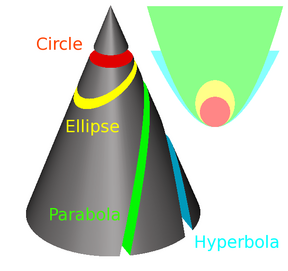
\includegraphics[width=0.5\textwidth, height=0.6\textheight, keepaspectratio]{images/conics.png}
    \caption{Las secciones cónicas: círculo, elipse, parábola y hipérbola}
  \end{figure}
\end{frame}

\begin{frame}{Forma General de las Secciones Cónicas}
  \begin{definition}
    Una sección cónica es el lugar en el plano cartesiano $\mathbb{R}^2$ de una ecuación de la forma
    \begin{equation*}
      ax^2 + bxy + cy^2 + dx + ey + f = 0. \tag{1}
    \end{equation*}
  \end{definition}
  Se puede demostrar que esta ecuación representa uno de los siguientes:
  \begin{enumerate}
    \item el conjunto vacío
    \item un solo punto
    \item una o dos rectas
    \item una elipse
    \item una hipérbola, o
    \item una parábola.
  \end{enumerate}
  La parte de segundo grado de (1), $q(x, y) = ax^2 + bxy + cy^2$ es una forma cuadrática. Esto determina el tipo de la cónica.
\end{frame}

\begin{frame}{Forma Matricial de las Secciones Cónicas}
  \frametitle{Forma Matricial de las Secciones Cónicas}
  Podemos escribir la ecuación en forma matricial:
  \begin{equation*}
    [x, y] \begin{bmatrix} a & b/2 \\ b/2 & c \end{bmatrix} \begin{bmatrix} x \\ y \end{bmatrix} + [d, e] \begin{bmatrix} x \\ y \end{bmatrix} + f = 0.
  \end{equation*}
  Escribimos $A = \begin{bmatrix} a & b/2 \\ b/2 & c \end{bmatrix}$. Sea $U = [u, v]$ una matriz ortogonal cuyos vectores de columna $u$ y $v$ son vectores propios de $A$ con valores propios $\lambda_1$ y $\lambda_2$. Aplicamos el cambio de variables
  \begin{equation*}
    x = \begin{bmatrix} x \\ y \end{bmatrix} = U \begin{bmatrix} u \\ v \end{bmatrix}
  \end{equation*}
  para diagonalizar la forma cuadrática $q(x, y)$ a la forma diagonal
  \begin{equation*}
    \lambda_1u^2 + \lambda_2v^2.
  \end{equation*}
\end{frame}

\begin{frame}{Transformación de Coordenadas}
  \frametitle{Transformación de Coordenadas}
  La base ortonormal \{u, v\} determina un nuevo conjunto de ejes de coordenadas con respecto a los cuales el lugar de la ecuación
  \begin{equation*}
    [x, y] A [x, y]^T + B [x, y]^T + f = 0
  \end{equation*}
  con B = [d, e] es el mismo que el lugar de la ecuación
  \begin{equation*}
    0 = [u, v] \text{diag} (\lambda_1, \lambda_2) [u, v]^T + (BU) [u, v]^T + f
  \end{equation*}
  por lo tanto
  \begin{equation*}
    \lambda_1 u^2 + \lambda_2 v^2 + [d, e] [u, v] [u, v]^T + f = 0 \tag{2}
  \end{equation*}
\end{frame}

\begin{frame}{Determinación del Tipo de Cónica}
  \frametitle{Determinación del Tipo de Cónica}
  Si la cónica determinada por (2) no es degenerada, es decir, no es un conjunto vacío, un punto, ni línea(s), entonces los signos de $\lambda_1$ y $\lambda_2$ determinan si es una parábola, una hipérbola o una elipse. La ecuación (1) representará
  \begin{itemize}
    \item una elipse si $\lambda_1\lambda_2 > 0$,
    \item una hipérbola si $\lambda_1\lambda_2 < 0$,
    \item una parábola si $\lambda_1\lambda_2 = 0$.
  \end{itemize}
\end{frame}

\begin{frame}{Bibliografia}
  \begin{itemize}
    \item \faGlobe\, Applications of Linear Algebra in Various Fields (Part-1): \url{https://www.researchgate.net/publication/356818396_Applications_of_Linear_Algebra_in_Various_Fields_Part-1}
    \item \faBook\, Álgebra lineal y geometría cartesiana - Juan de Burgos Román
    \item \faBook\, Practical Linear Algebra: A Geometry Toolbox - Gerald Farin, Dianne Hansford
  \end{itemize}
\end{frame}

\begin{frame}[standout]
  Gracias \\
\end{frame}

\end{document}